\lecture{4}

We will now discuss topological spaces based on our previous development of set theory. As we will see, a topology on a set provides the weakest structure in order to define the two very important notions of convergence of sequences to points in a set, and of continuity of maps between two sets.

\section{Topological Spaces}

\begin{definition}[Topology \& Topological Space]
	Let \(M\) be a set. Then a choice of subsets \(\O \subseteq \powerset(M)\) is called a \emph{topology} on \(M\) if
	\begin{enumerate}[(i)]
		\item \(\0 \in \O\) and \(M \in \O\),
		\item \(U, V \in \O \implies \bigcap \qty{U, V} \in \O\),
		\item \(C \subseteq \O \implies \bigcup C \in \O\).
	\end{enumerate}
	The pair \((M, \O)\) is then called a \emph{topological space}.
\end{definition}
\begin{remark}[Open \& Closed Sets]
	Let \((M, \O)\) be a topological space. Then
	\begin{enumerate}[(a)]
		\item A set \(U \in \O\) is called an \emph{open set} in \((M, \O)\).
		\item A set \(C \subseteq M\) is called a \emph{closed set} in \((M, \O)\) if \(M \setminus C \in \O\) \ie\ \(M \setminus C\) is open in \((M, \O)\).
	\end{enumerate}
\end{remark}

\begin{remark}[choice of topology]
	Unless \(\abs{M} = 1\), there are different topologies \(\O\) one can choose on one and the same set \(M\). Based on the choice of topology \(\O\), the notion of convergence of sequences and continuity of maps will change.
\end{remark}
For finite set, we can count the number of topologies on it.
\begin{table}[H]
	\centering
	\begin{tabular}{c|c}
		\toprule
		\(\abs{M}\) & Number of Topologies \\
		\midrule
		1           & 1                    \\
		2           & 4                    \\
		3           & 29                   \\
		4           & 355                  \\
		5           & 6,942                \\
		6           & 209,527              \\
		7           & 9,535,241            \\
		\vdots      & \vdots               \\
		\bottomrule
	\end{tabular}
\end{table}

\begin{example}[Basic Topologies]
	Let \(M\) be any set, then we can define following ``trivial'' topologies on \(M\):
	\begin{enumerate}[(a)]
		\item \(\O = \qty{\0, M}\). It is easy to see that, \(\O\) is a topology on \(M\). This is called the \emph{chaotic topology}.

		\item \(\O = \powerset(M)\). It is easy to see that, \(\O\) is a topology on \(M\). This is called the \emph{discrete topology}.
	\end{enumerate}
\end{example}
For a less abstract example, consider \(M = \qty{1, 2, 3}\), then we can define 29 different topologies on \(M\). For example, \(\O = \qty{\0, \qty{1}, \qty{2}, \qty{1, 2}, \qty{1, 2, 3}}\) is a topology on \(M\).

\begin{example}[Standard Topology on \(\R^d\)]
	This is the most important and heavily used topology in mathematics and physics.\\
	Consider \(M = \R^d\), where \(d \in \N\). Then the \emph{standard topology} on \(\Ostd\) is constructed as follows:
	\begin{equation*}
		U \in \Ostd :\iff \forall p \in U: \exists r \in \R^+: B_r(p) \subseteq U \label{eq:standard_topology}
	\end{equation*}
	where \(B_r(p) = \qty{x \in \R^d \mid \norm{x - p} < r}\) is the open ball of radius \(r\) around \(p\). In more involved terms, we can write the definition of the standard topology on \(\R^d\) as
	\begin{equation*}
		\Ostd = \qty{U \in \powerset(\R^d) \mid \forall p \in U: \exists r \in \R^+: B_r(p) \subseteq U} \label{eq:standard_topology_explicit}
	\end{equation*}
	Then by \cref{thm:PRC}, \(\Ostd\) is a set. Now we have to prove that \(\Ostd\) is indeed a topology on \(\R^d\).
	\begin{enumerate}[(i)]
		\item First, we need to check whether \(\0 \in \Ostd\), \ie\ whether:
		      \begin{equation*}
			      \forall p \in \0 : \exists r \in \R^+ : B_r(p) \subseteq \0
		      \end{equation*}
		      is true. This proposition is of the form \(\forall p \in \0 : Q(p)\), which was defined as being equivalent to:
		      \begin{equation*}
			      \forall p : p \in \0 \implies Q(p).
		      \end{equation*}
		      However, since \(p \in \0\) is false, the implication is true independent of \(p\). Hence, the initial proposition is true and thus \(\0 \in \Ostd\).

		      Second, by definition, we have \(B_r(x) \subseteq \R^d\) independent of \(x\) and \(r\), hence:
		      \begin{equation*}
			      \forall p \in \R^d : \exists r \in \R^+ : B_r(p) \subseteq \R^d
		      \end{equation*}
		      is true and thus \(\R^d\in\Ostd\).

		\item Let \(U, V \in \Ostd\), then we have to show that \(U\cap V\in\Ostd\). Let \(p \in U\cap V\), then \(p \in U\) and \(p \in V\). Since \(U, V \in \Ostd\), we have:
		      \begin{align*}
			      \exists r_1 \in \R^+ : B_{r_1}(p) & \subseteq U, \\
			      \exists r_2 \in \R^+ : B_{r_2}(p) & \subseteq V.
		      \end{align*}
		      Now, let \(r = \min\qty{r_1, r_2}\), then we have \(B_r(p) \subseteq B_{r_1}(p) \subseteq U\) and \(B_r(p) \subseteq B_{r_2}(p) \subseteq V\). Hence, \(B_r(p) \subseteq U\cap V\) and thus \(U\cap V\in\Ostd\).

		\item Let \(C \subseteq \Ostd\), then we have to show that \(\bigcup C\in\Ostd\). Let \(p \in \bigcup C\), then \(p \in U\) for some \(U \in C\). Since \(U \in \Ostd\), we have:
		      \begin{equation*}
			      \exists r \in \R^+ : B_r(p) \subseteq U \subseteq \bigcup C.
		      \end{equation*}
		      Hence, \(\bigcup C \in \Ostd\).
	\end{enumerate}
	Thus, \(\Ostd\) is a topology on \(\R^d\).
\end{example}

\begin{definition}[Comparison of Topologies]
	Let \(M\) be a set and \(\O_1, \O_2\) be two topologies on \(M\). If \(\O_1 \subseteq \O_2\), then we say that \(\O_2\) is \emph{finer} (or \emph{stronger}) topology than \(\O_1\), and \(\O_1\) is \emph{coarser} (or \emph{weaker}) topology than \(\O_2\).
\end{definition}
From this definition, we can see that the chaotic topology is the coarsest topology on a set, and the discrete topology is the finest topology on a set.

\pagebreak
\section{Construction of new Topologies from given topologies}

\subsection{Induced Topology}
\begin{theorem}[Induced Topology]\label{thm:induced_topology}
	Let \((M, \O)\) be a topological space and \(N \subset M\)\footnotemark. Then the following set
	\begin{equation}
		\eval{\O}_N = \qty{U \cap N \mid U \in \O} \subseteq \powerset(N) \label{eq:induced_topology}
	\end{equation}
	is a topology on \(N\), called the \emph{induced topology} on \(N\).
\end{theorem}
\footnotetext{We will use either \(N \subset M\) or \(N \subsetneq M\) or \(N \subsetneqq M\) to denote that \(N\) is a proper subset of \(M\).}

\begin{proof}
	We have to show that \(\eval{\O}_N\) is a topology on \(N\).
	\begin{enumerate}[(i)]
		\item First, as \(\0 \in \O\), we have \(\0 \cap N = \0 \in \eval{\O}_N\).

		      Second, since \(M \in \O\), we have \(M \cap N = N \in \eval{\O}_N\).

		\item \(U, V \in \eval{\O}_N \xRightarrow{?} U \cap V \in \eval{\O}_N\). From \eqref{eq:induced_topology}, \(\exists U_1, V_1 \in \O: U = U_1 \cap N \land V = V_1 \cap N\). Then we have:
		      \begin{equation*}
			      U \cap V = (U_1 \cap N) \cap (V_1 \cap N) = (U_1 \cap V_1) \cap N \in \eval{\O}_N
		      \end{equation*}
		      as \(U_1 \cap V_1 \in \O\).

		\item \(C \subseteq \eval{\O}_N \xRightarrow{?} \bigcup C\in\eval{\O}_N\). Since \(C \subseteq \eval{\O}_N\), we have \(C = \qty{U_i \cap N \mid U_i \in \O}\). Then we have:
		      \begin{equation*}
			      \bigcup C = \bigcup \qty{U_i \cap N \mid U_i \in \O} = \qty{\bigcup U_i} \cap N \in \eval{\O}_N.
		      \end{equation*}
	\end{enumerate}
	Thus, \(\eval{\O}_N\) is a topology on \(N\).
\end{proof}

\begin{example}
	Consider \((\R, \Ostd)\) and \(N = \qty[0, 1] := \qty{x \in \R \mid 0 \le x \le 1}\). Then from \cref{thm:induced_topology}, \((N, \eval{\Ostd}_N)\) is a topological space.

	It is easy to see that \((0, 1] \notin \Ostd\) so \((0, 1]\) is not open in \((\R, \Ostd)\), but \((0, 1] = (0, 2) \cap N \in \eval{\Ostd}_N\). Hence, \((0, 1]\) is an open set in \((N, \eval{\Ostd}_N)\).
\end{example}
At this point we can talk about openness and closedness of sets in a topological space.
\begin{remark}
	Let \((M, \O)\) be a topological space and \(N \subset M\). Then \(N\) is either
	\begin{itemize}[noitemsep]
		\item open, or
		\item closed, or
		\item open and closed, or
		\item open and not closed, or
		\item not open and closed, or
		\item not open and not closed.
	\end{itemize}
\end{remark}
For this very unintuitive idea of a set to be open and closed at the same time, see the following example.
\begin{example}
	For any topological space \((M, \O)\), we know by definition of topology that \(\0, M \in \O\). Hence, \(\0\) and \(M\) are open in \((M, \O)\).
	\begin{itemize}
		\item Now, let \(N = M\), then \(M \setminus N = \0 \in \O\). Hence, \(M\) is closed in \((M, \O)\).
		\item Let \(N = \0\), then \(M \setminus N = M \in \O\). Hence, \(\0\) is closed in \((M, \O)\).
	\end{itemize}
	Thus, \(\0\) and \(M\) are both open and closed in \((M, \O)\).
\end{example}
\subsection{Quotient Topology}
\begin{definition}[Quotient Topology]\label{def:quotient_topology}
	Let \((M, \O)\) be a topological space and \(\sim\) be an equivalence relation on \(M\). Then the quotient set \(\faktor{M}{\sim}\) can be equipped with the \emph{quotient topology} \(\Oq{M}\) defined as follows:
	\begin{equation}
		\Oq{M} = \qty{U \subseteq \faktor{M}{\sim} \mid \bigcup U = \bigcup_{[u] \in U} [u] \in \O} \label{eq:quotient_topology}
	\end{equation}
\end{definition}
An equivalent definition of the quotient topology is as follows: Let \(\pi: M \to \faktor{M}{\sim}\) be the map defined as \(\pi(m) = [m]\). Then the quotient topology is defined as
\begin{equation}
	\Oq{M} = \qty{U \subseteq \faktor{M}{\sim} \mid \preimg_{\pi}(U) \in \O} \label{eq:quotient_topology_map}
\end{equation}

\begin{example}[Topology on 1-sphere]
	Consider \(M = \R^2\). The \emph{circle} (or \emph{1-sphere}) is defined as a set \(S^1 := \qty{(x, y) \in \R^2 \mid x^2 + y^2 = 1}\). We have two ways to construct a new topological space:
	\begin{enumerate}[(a)]
		\item \uline{Induced Topology:} As \(S^1 \subset \R^2\), we can construct a topology \(\O\) on \(S^1\) by \cref{thm:induced_topology} using \((\R^2, \Ostd)\) topological space. This is the \emph{standard topology} on \(S^1\).
		      \begin{figure}[H]
			      \centering
			      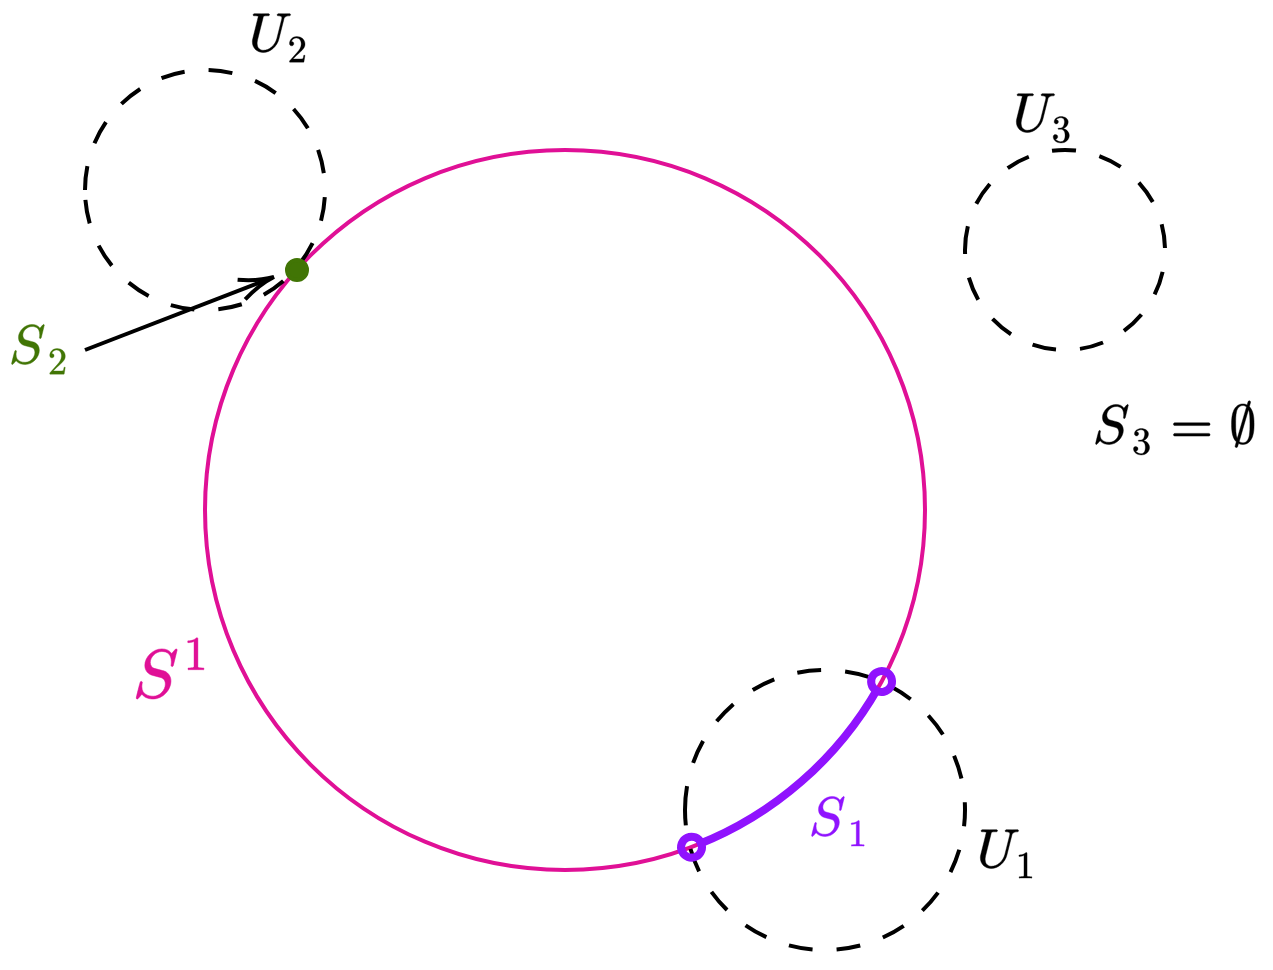
\includegraphics[width=0.35\textwidth]{lec04-1_sphere.png}
			      \caption{1-sphere induced topology}
			      \label{fig:1-sphere_induced_topology}
		      \end{figure} \noindent
		      From \cref{fig:1-sphere_induced_topology}, we can see that \(U_i\)'s are open in \(\R^2\) and \(U_i \cap S^1\) are open in \(S^1\). See, \(U_3 \in \Ostd \implies \0 \in \O\) and \(U_1 \in \Ostd \implies S_1 \in \O\). Also the set \(S_2\) is not open in \(S^1\) as \(\forall U \in \powerset(\R): U \cap S^1 \neq S_2\). Hence, \(S_2 \notin \O\).

		\item \uline{Quotient Topology:} Let $\sim$ be the equivalence relation on $\R$ defined by:
		      \begin{equation*}
			      x \sim y :\iff \exists n \in \Z : x = y + 2 \pi n.
		      \end{equation*}
		      Then the circle can be defined as the set $S^1 := \faktor{\R}{\sim}$ equipped with the quotient topology.
	\end{enumerate}
\end{example}

\subsection{Product Topology}

\begin{definition}[Product Topology]
	Let \((A, \O_A)\) and \((B, \O_B)\) be two topological spaces. Then the set \(\O_{A \times B}\) defined implicitly as
	\begin{equation}
		U \in \O_{A \times B} :\iff \forall (a, b) \in U: \exists U_A \in \O_A, U_B \in \O_B: a \in U_A \land b \in U_B \land U_A \times U_B \subseteq U \label{eq:product_topology}
	\end{equation}
	is a topology on \(A \times B\), called the \emph{product topology} on \(A \times B\).
\end{definition}
Here we used the existence of \(U_A\) and \(U_B\) such that it contains \(a\) and \(b\) respectively. And we will use this kind of argument throughout our discussion.

\noindent Let \((M, \O)\) be a topological space. Let \(a \in M\) be a point. Then we say that a set \(U \in \O\) is an \emph{open neighbourhood} of \(a\) if \(a \in U\).

Intuitively, the definition can be understood with the help of following diagram:
\begin{figure}[H]
	\centering
	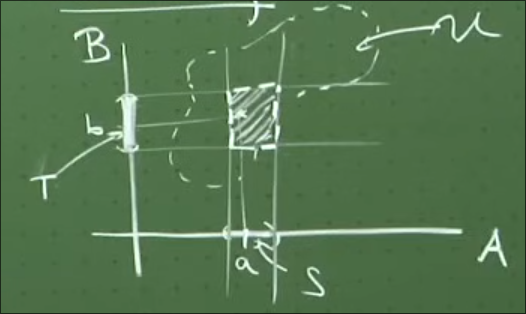
\includegraphics[width=0.375\textwidth]{lec04-prod_topology_intuition.png}
	% \caption{Product Topology Intuition}
	\label{fig:prod_topology_intuition}
\end{figure}

\begin{remark}[Extending product topology to finite cartesian product]
	Let \(A_1, A_2, \ldots, A_N\) be topological spaces. Then in same spirit, we can define the product topology
	\begin{equation*}
		\O_{A_1 \times A_2 \times \cdots \times A_N}
	\end{equation*}
\end{remark}
With this, we can check that the standard topology on \(\R^d\) is a product topology with open ball defined using \(\norm{\cdot}_{\infty}\)
\begin{equation*}
	\Ostd {\;}_{\R^d} = \O_{\underbrace{\R \times \R \times \cdots \times \R}_{d\ \text{times}}}
\end{equation*}

Till this point, we have seen topology and topological spaces from geometric view-point. But one can use these things beyond the geometric (or manifold) applications. For example, a guy named Furstenberg introduced a simple topology on the set of integers to prove the infinitude of primes.

\section{Convergence}

\begin{definition}[Sequence]
	A \emph{sequence} (of points) in a set \(M\) is a map from \(\N\) onto \(M\), \ie\ \(q: \N \to M\).
\end{definition}

\begin{definition}[Convergence and Limit Point]
	Let \((M, \O)\) be a topological space. A sequence \(q\) in \(M\) is said to \emph{converge} against a \emph{limit point} \(a \in M\) if
	\begin{equation}
		\forall U \in \O: a \in U \implies \exists N \in \N: \forall n > N: q(n) \in U \label{eq:convergence}
	\end{equation}
\end{definition}

\begin{example}[Justifying different topologies]
	With the notion of convergence, we can justify the different topologies on a set.
	\begin{enumerate}[(a)]
		\item \uline{Chaotic Topology:} Consider the chaotic topology \(\O = \qty{\0, M}\) on \(M\). Then any sequence in \(M\) converges against any point in \(M\). Let \(a \in M\) and \(q\) be a sequence in \(M\), then we have only two choice for \(U \in \O\), \ie\ \(U = \0\) or \(U = M\). In case \(U = \0\), the definition of convergence is vacuously true. In case \(U = M\), the definition of convergence is true as \(q(n) \in M\) for all \(n \in \N\). Hence, (arbitrary) sequence \(q\) converges against (arbitrary) point \(a\) in \((M, \O)\).

		      This weird behavior is the reason for the name ``chaotic topology''.

		\item \uline{Discrete Topology:} Consider the discrete topology \(\O = \powerset(M)\) on \(M\). Then only almost constant sequences converge against a (unique) point in \(M\). Let \(a \in M\) and \(q\) be a sequence in \(M\), then we have \(U = \qty{a} \in \O\). Then the definition of convergence is true if and only if \(q(n) = a\) for all \(n > N\). Hence, only almost constant sequences converge against a point in \((M, \O)\).
	\end{enumerate}
\end{example}

Here we can see that every sequence is convergent in chaotic topology (the coarsest topology) and only a specific kind of sequence is convergent in discrete topology (the finest topology). So we deduce the following remark.

\begin{remark}\label{rem:convergence_in_comparison_topologies}
	Let \(M\) be a set and \(\O_1, \O_2\) be two topologies on \(M\) such that \(\O_1 \subseteq \O_2\) and let \(q\) be a sequence in \(M\). Then if \(q\) converges in \((M, \O_2)\), then \(q\) converges in \((M, \O_1)\) but not necessarily vice-versa.
\end{remark}

\begin{theorem}[Convergence in standard topology on \(\R^d\)]
	Let \(q\) be a sequence in \(\R^d\) and \(a \in \R^d\). Then \(q\) converges against \(a\) in \((\R^d, \Ostd)\) if and only if
	\begin{equation}
		\forall \eps > 0: \exists N \in \N: \forall n > N: \norm{q(n) - a} < \eps \label{eq:convergence_Rd}
	\end{equation}
\end{theorem}

\begin{proof}
	Let \(q\) be a sequence in \(\R^d\) and \(a \in \R^d\). Then \(q\) converges against \(a\) in \((\R^d, \Ostd)\) if and only if
	\begin{equation}
		\forall U \in \Ostd: a \in U \implies \exists N \in \N: \forall n > N: q(n) \in U \label{eq:convergence_Rd_1}
	\end{equation}
	From the definition of standard topology on \(\R^d\), we have \(U \in \Ostd \implies \exists r \in \R^+: B_r(a) \subseteq U\). Hence, \eqref{eq:convergence_Rd_1} is equivalent to
	\begin{equation}
		\forall r > 0: \exists N \in \N: \forall n > N: q(n) \in B_r(a) \label{eq:convergence_Rd_2}
	\end{equation}
	which is equivalent to \eqref{eq:convergence_Rd}.
\end{proof}

\begin{example}[Convergence in \(\R\)]
	Let \(q(n) = 1 - \frac{1}{n + 1}\) be a sequence in \(\R\). Then \(q\) converges against \(1\) in \((\R, \Ostd)\) as
	\begin{equation*}
		\forall \eps \in \R^+: \exists N \in \N: \forall n > N: \abs{q(n) - 1} = \abs{1 - \frac{1}{n + 1} - 1} = \frac{1}{n + 1} < \eps
	\end{equation*}
	But observe \(q\) is not almost constant sequence and hence does not converge in \((\R, \powerset(\R))\).
\end{example}

\section{Continuity}

\begin{definition}[Continuity]
	Let \((M, \O_M)\) and \((N, \O_N)\) be two topological spaces and \(\phi: M \to N\) be a map. Then \(\phi\) is said to be \emph{continuous} if
	\begin{equation}
		\forall V \in \O_N: \preimg_{\phi}(V) \in \O_M \label{eq:continuity}
	\end{equation}
	In other words, \(\phi\) is continuous iff the pre-image of every open set in \(N\) is open in \(M\).
\end{definition}

\begin{example}[`Trivial' Continuity]
	Let \((M, \O_M)\) and \((N, \O_N)\) be two topological spaces and \(\phi: M \to N\) be a map. Then
	\begin{enumerate}[(a)]
		\item Let \(\O_M = \powerset(M)\) and \(\O_N\) be any topology on \(N\). Then every map is continuous.

		      Let \(V \in \O_N\) be any open set in \(N\). Then \(\preimg_{\phi}(V) \subseteq M\) and hence \(\preimg_{\phi}(V) \in \O_M\). Hence, \(\phi\) is continuous.

		\item Let \(\O_M\) be any topology on \(M\) and \(\O_N = \qty{\0, N}\). Then every map is continuous.

		      Here, either \(V = \0\) or \(V = N\). In case \(V = \0\), we have \(\preimg_{\phi}(\0) = \0 \in \O_M\). In case \(V = N\), we have \(\preimg_{\phi}(N) = M \in \O_M\). Hence, \(\phi\) is continuous.
	\end{enumerate}
\end{example}

Recovering the definition of \(\eps-\delta\) definition of continuity on `Euclidean' spaces from the definition of continuity in topological spaces.
\begin{theorem}[Continuity in Euclidean spaces]
	Let \(f: \R^m \to \R^n\) be a map. Then \(f\) is continuous if and only if
	\begin{equation}
		\forall a \in \R^m: \forall \eps > 0: \exists \delta > 0: \norm{x - a} < \delta \implies \norm{f(x) - f(a)} < \eps \label{eq:continuity_Rm_Rn}
	\end{equation}
\end{theorem}

\begin{proof}
	Let \(f: \R^m \to \R^n\) be a map. Then \(f\) is continuous if and only if
	\begin{equation}
		\forall U \in \O_{\R^n}: \preimg_{f}(U) \in \O_{\R^m} \label{eq:continuity_Rm_Rn_1}
	\end{equation}
	From the definition of standard topology on \(\R^n\), we have \(U \in \O_{\R^n} \implies \exists \eps > 0: B_{\eps}(f(a)) \subseteq U\). Hence, \eqref{eq:continuity_Rm_Rn_1} is equivalent to
	\begin{equation}
		\forall \eps > 0: \exists \delta > 0: \preimg_{f}(B_{\eps}(f(a))) \in \O_{\R^m} \label{eq:continuity_Rm_Rn_2}
	\end{equation}
	which is equivalent to \eqref{eq:continuity_Rm_Rn}.
\end{proof}

\subsection{Homeomorphism}

\begin{definition}[Homeomorphism]
	Let \((M, \O_M)\) and \((N, \O_N)\) be two topological spaces. Let \(\phi: M \to N\) be a bijection. Then \(\phi\) is said to be a \emph{homeomorphism} if
	\begin{enumerate}[(a)]
		\item \(\phi\) is continuous, and
		\item \(\phi^{-1}\) is continuous.
	\end{enumerate}
\end{definition}

\begin{remark}[Structure preserving maps]
	Homeo(morphism)s are structure preserving maps in topology.
\end{remark}

\begin{remark}[One-to-one pairing of open sets]
	Let \((M, \O_M)\) and \((N, \O_N)\) be two topological spaces and let \(\phi: M \to N\) be a homeomorphism.
	\begin{figure}[H]
		\centering
		\begin{tikzcd}
			M \arrow[r, bend left, "\phi"] & N \arrow[l, bend left, "\phi^{-1}"]
		\end{tikzcd}
	\end{figure}
	Then \(\phi\) provides a \emph{one-to-one} pairing of the open sets of \(M\) with those of \(N\).
\end{remark}

\begin{definition}[Homeomorphic]
	Let \((M, \O_M)\) and \((N, \O_N)\) be two topological spaces. Then \(M\) and \(N\) are said to be \emph{homeomorphic} if there exists a homeomorphism between them. And we write
	\begin{equation}
		M \topIso N \label{eq:homeomorphic}
	\end{equation}
\end{definition}

\begin{remark}[Homeomorphic \& Isomorphic]
	Let \((M, \O_M)\) and \((N, \O_N)\) be two homeomorphic topological spaces. Then they are isomorphic as sets. But the converse is not true.
	\begin{equation}
		M \topIso N \implies M \setIso N \label{eq:homeomorphic_isomorphic}
	\end{equation}
\end{remark}
